% Bearbeitbare Hauptdatei der Bedienungsanleitung.
% Im Ordner docs zweimal kompilieren:
%   pdflatex benutzerhandbuch-de.tex
% Alternativ im Projektstamm:
%   python scripts/build_user_manual.py
% Benötigt eine übliche LaTeX-Installation mit deutscher Sprachunterstützung.

\documentclass[a4paper,11pt]{article}

\usepackage[T1]{fontenc}
\usepackage[utf8]{inputenc}
\usepackage[ngerman]{babel}
\usepackage{lmodern}
\usepackage{microtype}
\usepackage[left=24mm,right=24mm,top=24mm,bottom=24mm,headheight=15pt]{geometry}
\usepackage{graphicx}
\usepackage{booktabs}
\usepackage{tabularx}
\usepackage{array}
\usepackage{fancyhdr}
\usepackage[hidelinks]{hyperref}

\hypersetup{
  pdftitle={Measure Shift -- Bedienungsanleitung: Bildausrichtung mit dem Joystick},
  pdfsubject={Referenzaufnahme, Pixelkalibrierung, X-Ausrichtung und schrittweises Verfahren},
  pdfauthor={},
  pdflang={de-DE}
}

\setlength{\parindent}{0pt}
\setlength{\parskip}{0.5em}
\setlength{\emergencystretch}{1.5em}
\renewcommand{\arraystretch}{1.15}
\newcolumntype{Y}{>{\raggedright\arraybackslash}X}
\newcolumntype{L}[1]{>{\raggedright\arraybackslash}p{#1}}

\pagestyle{fancy}
\fancyhf{}
\fancyhead[L]{\small Measure Shift}
\fancyhead[R]{\small Bedienungsanleitung}
\fancyfoot[L]{\small Ausgabe: 16.11.2026}
\fancyfoot[R]{\small Seite \thepage\ von \pageref*{LastPage}}
\renewcommand{\headrulewidth}{0.4pt}
\renewcommand{\footrulewidth}{0.4pt}

% Diese Bezeichnungen beschreiben Funktionen am Joystick, keine Tastenpositionen.
\newcommand{\Referenz}{\textbf{Referenztaster}}
\newcommand{\Ausrichten}{\textbf{Ausrichttaster}}
\newcommand{\Status}[1]{\texttt{#1}}
\newcommand{\Hinweis}[2]{\par\smallskip\textbf{#1}\enspace #2\par\smallskip}

\begin{document}

\begin{center}
  {\LARGE\bfseries Measure Shift\par}
  \medskip
  {\Large Bedienungsanleitung\par}
  \smallskip
  {\large Bildausrichtung mit dem Joystick\par}
\end{center}

\section{Voraussetzungen und Bedienelemente}

Diese Anleitung setzt eine Livekamera, eine eingerichtete Achsensteuerung
und aktivierte Joystick-Funktionen voraus. Die Achsensteuerung legt den
Verfahrweg pro Relaisimpuls fest. Stellen Sie die gewünschte Bildtoleranz
in der Anwendung ein.

\begin{tabularx}{\linewidth}{@{}L{0.28\linewidth}Y@{}}
\toprule
\textbf{Bedienelement} & \textbf{Funktion} \\
\midrule
Joystick links/rechts & Die Motorachse schrittweise verfahren. Halten wiederholt die Bewegung. \\
\Referenz & Das aktuelle Kamerabild als neues Sollbild übernehmen. \\
\Ausrichten{} oder \textbf{Align X} & Die direkte X-Ausrichtung am aktuellen Sollbild starten. \\
\textbf{Run pixel calibration} & Den X-Versatz pro Relaisimpuls messen. \\
\bottomrule
\end{tabularx}

Die Bezeichnungen benennen die zugeordneten Funktionen am Joystick. Die genaue
Lage der Taster richtet sich nach Ihrem Aufbau.

\section{Arbeitsablauf}

\begin{enumerate}
  \setlength{\itemsep}{0.45em}
  \item \textbf{Bereitschaft prüfen.} Prüfen Sie, ob sich das Livebild aktualisiert und die
  Achse bereit ist.

  \item \textbf{Referenz aufnehmen.} Nach Stillstand den \Referenz{} einmal drücken
  und loslassen. Links muss nun das gewünschte Sollbild erscheinen.

  \item \textbf{Teil vorpositionieren.} Das auszurichtende Teil mit dem
  Joystick schrittweise verfahren, bis das Merkmal im Bild gut sichtbar ist.
  Danach den Joystick loslassen und Stillstand abwarten.

  \item \textbf{Ausrichten.} Den \Ausrichten{} einmal drücken und loslassen.
  Während der automatischen Korrekturen den Joystick in Neutralstellung lassen.

  \item \textbf{Ergebnis kontrollieren.} Die Achsenmeldung
  \Status{X aligned}, die X/Y-Werte und die Bildüberdeckung prüfen.
  Die Gesamtanzeige \Status{ALIGNED} bestätigt den Bildversatz innerhalb der
  eingestellten Toleranz.
\end{enumerate}

\newpage
\section{Bildschirmkontrolle}

Links zeigt \textbf{REFERENCE} das feste Sollbild. Rechts zeigt \textbf{LIVE}
das aktuelle Kamerabild. Unter \textbf{Alignment} stehen der Messstatus,
die X/Y-Abweichung und die vorbereitete Toleranz.

\begin{center}
  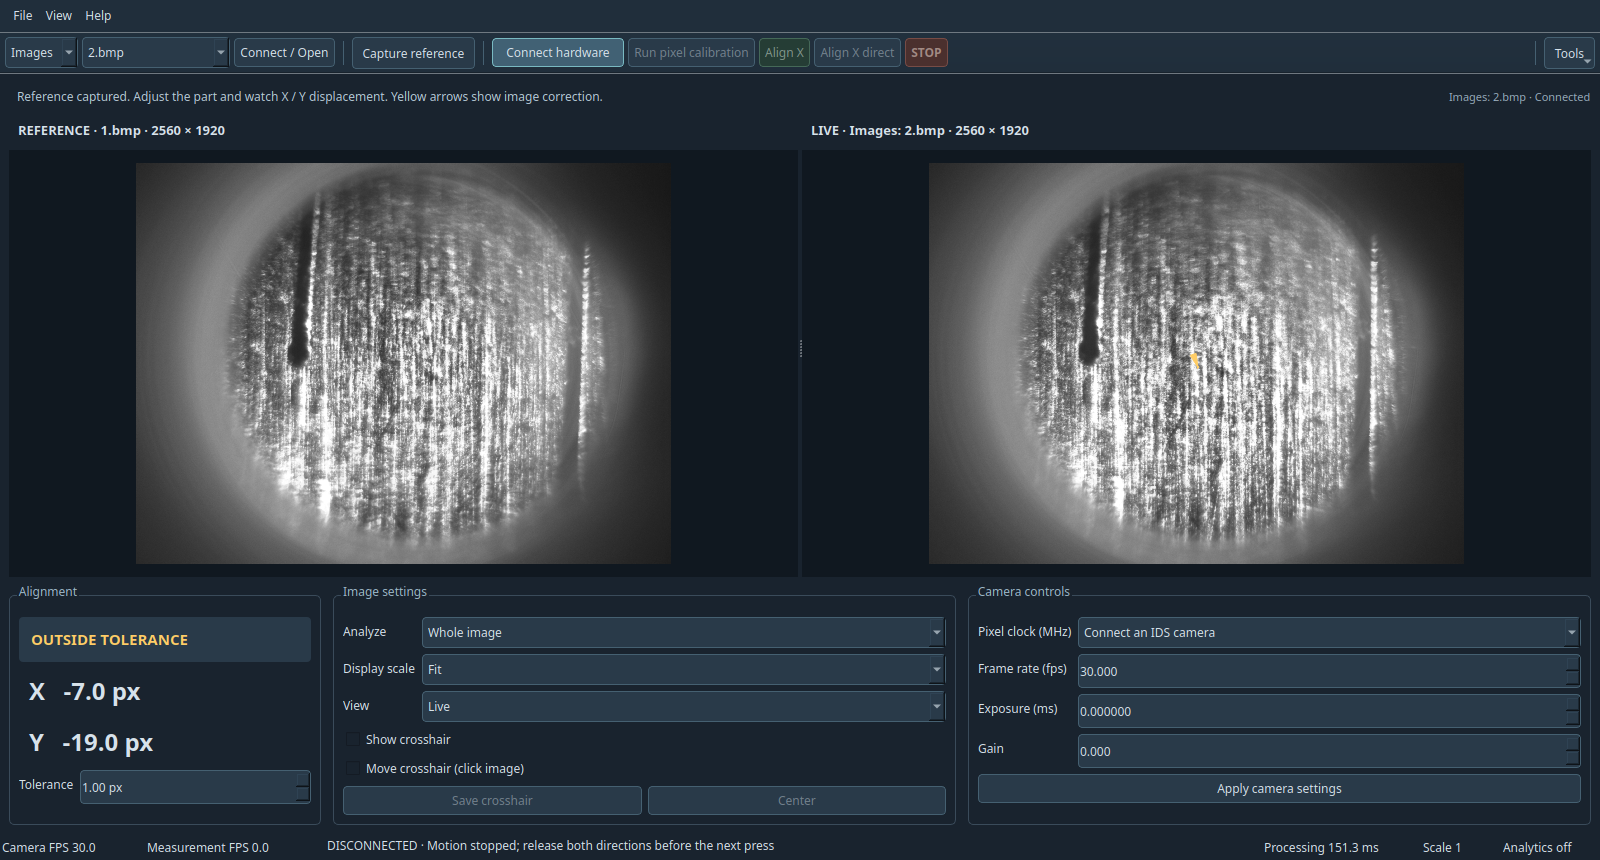
\includegraphics[width=0.90\linewidth]{assets/bedienoberflaeche.png}
  \par\smallskip
  {\small\textbf{Abbildung 1:} Bildschirmübersicht mit gespeicherten
  Beispielbildern. Die Bedienung im beschriebenen Arbeitsablauf erfolgt am Joystick.}
\end{center}

\subsection{X- und Y-Abweichung}

Die Werte geben den Versatz des aktuellen Bildinhalts zum Sollbild in
Bildpixeln (px) an. X ist waagerecht, Y senkrecht.

\begin{tabularx}{\linewidth}{@{}L{0.22\linewidth}Y@{}}
\toprule
\textbf{Messwert} & \textbf{Bedeutung im Bild} \\
\midrule
X positiv / negativ & Nach rechts / nach links versetzt. \\
Y positiv / negativ & Nach unten / nach oben versetzt. \\
\bottomrule
\end{tabularx}

Der gelbe Pfeil zeigt die benötigte Korrekturrichtung im Bild. Welche
Joystick-Richtung den Bildinhalt nach links oder rechts bewegt, hängt vom
eingerichteten Aufbau ab. Beobachten Sie die Wirkung zunächst bei einer kleinen
Bewegung.

\subsection{Ausrichtung beurteilen}

\Hinweis{Korrektur der X-Achse.}{Die Motorachse korrigiert ausschließlich
X. Ein verbleibender Y-Versatz wird mit diesem Joystick-Ablauf nicht korrigiert.
Liegt Y außerhalb der Vorgabe, ist die Einrichtung zu prüfen.}

Die eingestellte \textbf{Tolerance} gilt für den gesamten Abstand aus X und Y.
Bei einer Toleranz von 1~px liegen beispielsweise X~=~0,8~px und Y~=~0,8~px
zusammen noch außerhalb. Maßgeblich ist der Status; die Zahlenanzeige ist leicht
geglättet.

\Hinweis{Rechnerische Vorschau.}{Ansichten mit \textbf{Compensated} verschieben
das Bild nur rechnerisch. Eine passende Vorschau bestätigt deshalb keine
mechanische Ausrichtung. Prüfen Sie die Messwerte und die tatsächliche Überdeckung.}

\newpage
\section{Bedienhinweise für den Joystick}

\subsection{Schrittweise verfahren}

Lenken Sie den Joystick kurz nach links oder rechts aus und lassen Sie ihn
wieder los. Ein erkannter Richtungsimpuls löst einen Verfahrschritt mit der
vorbereiteten Schrittweite aus. Halten wiederholt die Schritte nacheinander.
Nach dem Loslassen läuft nur der bereits begonnene Schritt zu Ende.

Warten Sie vor einem Richtungswechsel die Neutralstellung und den Stillstand
ab. Betätigungen, die vor der Bereitschaft bereits wieder losgelassen wurden,
werden nicht nachträglich ausgeführt.

\subsection{Referenz aufnehmen}

Den \Referenz{} bei stillstehendem Teil einmal drücken und wieder loslassen.
Halten erzeugt keine weiteren Aufnahmen. Zwischen zwei Referenzaufnahmen muss
mindestens eine Sekunde liegen.

Eine neue Aufnahme ersetzt das bisherige Sollbild. Prüfen Sie deshalb die
Position vor der Aufnahme. Nehmen Sie nach einem Neustart die benötigte
Referenz wieder über den Joystick auf.

\subsection{Direkte X-Ausrichtung starten}

Drücken Sie den \Ausrichten{} einmal und lassen Sie ihn wieder los oder
klicken Sie auf \textbf{Align X}. Die Anwendung vergleicht den X-Versatz nach
jedem Relaisimpuls mit dem vorherigen Messwert und bestimmt daraus die
nächste Richtung. Halten startet einen einzelnen Vorgang. Warten Sie vor dem
nächsten Tastendruck das Ende des laufenden Vorgangs ab.

\subsection{Versatz pro Relaisimpuls messen}

\textbf{Run pixel calibration} ermittelt bei Bedarf den X-Versatz in Pixeln
pro Rechtsimpuls. Stellen Sie in \textbf{Motion Setup} unter \textbf{Test presses}
eine positive Anzahl für Rechtsimpulse oder eine negative für Linksimpulse ein.
Das Merkmal muss während der Messung sichtbar bleiben. Das Teil bleibt an der
Endposition.

\subsection{Laufenden Vorgang abbrechen}

Um eine laufende Kalibrierung oder automatische Ausrichtung abzubrechen,
lenken Sie den Joystick kurz in eine Fahrtrichtung aus und lassen Sie ihn
wieder los. Der automatische Vorgang wird abgebrochen. Warten Sie Stillstand
und Neutralstellung ab, bevor Sie erneut verfahren oder den \Ausrichten{}
betätigen. Das Loslassen des Ausrichttasters allein bricht einen laufenden
Vorgang nicht ab.

\newpage
\section{Statusmeldungen und Störungen}

Die Messanzeige und die Achsenmeldung beschreiben unterschiedliche Zustände.
Prüfen Sie bei einer Unterbrechung beide Anzeigen.

\begin{tabularx}{\linewidth}{@{}L{0.34\linewidth}Y@{}}
\toprule
\textbf{Anzeige} & \textbf{Bedeutung und nächster Schritt} \\
\midrule
\Status{ALIGNED} & Der gesamte Bildversatz liegt innerhalb der eingestellten Toleranz. Bildüberdeckung prüfen. \\
\addlinespace
\Status{X aligned} & X ist ausgerichtet. Zusätzlich Y und den Gesamtstatus prüfen. \\
\addlinespace
\Status{OUTSIDE TOLERANCE} & Der Gesamtversatz ist noch zu groß. Bei verbleibendem X-Versatz erneut mit dem Ausrichttaster ausrichten. Y wird nicht motorisch korrigiert. \\
\addlinespace
\Status{NO REFERENCE} & Das Sollbild fehlt. Sollposition herstellen und den Referenztaster am Joystick betätigen. \\
\addlinespace
\Status{MATCH UNCERTAIN} & Der Bildvergleich ist unsicher. Merkmal und Überdeckung prüfen, bei Bedarf mit dem Joystick vorsichtig vorpositionieren. Bleibt die Meldung bestehen, Einrichtung prüfen lassen. \\
\addlinespace
\Status{PAUSED} & Bild und Messung werden nicht aktualisiert. Die zuständige Person muss den laufenden Kamerabetrieb wiederherstellen. \\
\addlinespace
\Status{DISCONNECTED} / \Status{STALE MEASUREMENT} & Verbindung oder aktuelles Kamerabild fehlt. Mit diesen Messwerten keine Ausrichtung bestätigen. Verbindung und Einrichtung prüfen lassen. \\
\bottomrule
\end{tabularx}

\subsection{Ein Taster reagiert nicht}

Lassen Sie Joystick und Taster vollständig los. Warten Sie, bis die Achse
stillsteht und bereit ist. Betätigen Sie den gewünschten Taster danach erneut.
Ein während der Fahrt oder vor der Bereitschaft gedrückter Taster startet
später keinen Vorgang nachträglich. Bleibt die Reaktion aus, lassen Sie die
Joystick-Zuordnung und die Verbindung prüfen.

\subsection{Kalibrierung oder Ausrichtung wird nicht abgeschlossen}

Prüfen Sie, ob dasselbe gut erkennbare Merkmal im Bild bleibt und das Livebild
aktuell ist. Nach einem Abbruch den Joystick in Neutralstellung bringen und
die Achsenmeldung lesen. Bleibt die Ursache bestehen, die zuständige Person
für die Einrichtung hinzuziehen. Den \Referenz{} nicht zum Beseitigen einer
unerwünschten Abweichung betätigen; dadurch würde lediglich das Sollbild ersetzt.

\smallskip
\textbf{Analytics:} Für diesen Arbeitsablauf nicht erforderlich. Der
Analysebereich kann ausgeschaltet bleiben; die X/Y-Messung läuft weiter.

\label{LastPage}
\end{document}
